\section{Assemblaggio e flashing del dispositivo}
Questa sezione è una guida passo-passo per l'assemblaggio e la preparazione del dispositivo OpenLDAT.

\subsection{Assemblaggio}
Il dispositivo OpenLDAT è piuttosto semplice da assemblare, il processo richiede tra 15 e 60 minuti a seconda del livello di abilità di saldatura.

Prima di iniziare, bisogna preparare i seguenti strumenti:
\begin{itemize}
	\item Saldatore a stagno a 450°C
	\item Rotolo di stagno per saldatura, meglio se con flussante
	\item Tronchesino o strumento di taglio simile
	\item Una breadboard o altro strumento in cui tenere fermi i pin header mentre si salda
\end{itemize}

Attenzione: la qualità delle saldature influisce direttamente sulla qualità dei segnali che il dispositivo OpenLDAT sarà in grado di catturare.

Una volta preparati tutti gli strumenti, si possono preparare i materiali (figura \ref{fig:assembly_01}):
\begin{itemize}
	\item Board Sparkfun Pro Micro 5V/16MHz con header
	\item Sensore Adafruit ALS-PT19 con header
	\item PCB OpenLDAT Model 1 (stampato o fatto in casa)
	\item Resistenze (330k\si{\ohm}, 22k\si{\ohm}, 47k\si{\ohm}, 1k\si{\ohm}, 1k\si{\ohm})
	\item LED da 3mm
\end{itemize}

\paragraph{Passo 1} Saldare gli header sulla board Sparkfun Pro Micro, in modo che la parte in plastica e la parte lugna dei pin sia sotto alla board. Per tenere i pin fermi e dritti mentre si salda, è utile infilarli in una breadboard o in un soldering jig apposito, come in figura \ref{fig:assembly_02}.

\paragraph{Passo 2} Saldare gli header sul piccolo PCB del sensore ALS-PT19, in modo che la parte in plastica e la parte lunga dei pin sia sotto al PCB e il sensore sia sopra, come in figura \ref{fig:assembly_03}. Poiché il PCB è molto piccolo, bisogna prestare attenzione a non scaldarlo troppo col saldatore, altrimenti il sensore potrebbe danneggiarsi.

\paragraph{Passo 3} Sulla parte posteriore del PCB OpenLDAT (quella dove ci sono le piste), posizionare le resistenze nelle posizioni corrette, piegando le gambette per tenerle ferme come in figura \ref{fig:assembly_04}, dopodiché saldarle e tagliare l'eccesso con il tronchesino, come in figura \ref{fig:assembly_05}.\\
\textbf{Attenzione: se le resistenze non sono in posizione corretta, i livelli di gain del sensore saranno totalmente diversi da quelli che si aspetta l'applicazione, e questa produrrà risultati invalidi.}\\
Il seguente elenco riassume le resistenze che devono essere saldate sul dispositivo, con i relativi valori e codici dei colori:
\begin{itemize}
	\item R1: 1k\si{\ohm} (Marrone-Nero-Rosso)
	\item R2: 1M\si{\ohm} (Marrone-Nero-Verde)
	\item R3: 330k\si{\ohm} (Arancio-Arancio-Giallo)
	\item R4: 22k\si{\ohm} (Rosso-Rosso-Arancio)
	\item R5: 47k\si{\ohm} (Giallo-Viola-Arancio)
\end{itemize}

\paragraph{Passo 4} Posizionare il sensore ALS-PT19 sulla parte posteriore del PCB OpenLDAT come in figura \ref{fig:assembly_06} e saldarlo avendo cura di tenerlo in posizione parallela al PCB, dopodiché, usando il tronchesino, rimuovere i pin in eccesso come in figura \ref{fig:assembly_07}.

\paragraph{Passo 5} Sulla parte frontale del PCB OpenLDAT, posizionare la board Sparkfun Pro Micro con il connettore USB dallo stesso lato del sensore ALS-PT19 e posizionare il LED prestando attenzione alla polarità, piegando le gambette per tenerlo fermo, come in figura \ref{fig:assembly_08}, dopodiché saldare il tutto e usando il tronchesino, rimuovere i pin in eccesso dalla parte posteriore del PCB, come in figura \ref{fig:assembly_09}.

\paragraph{Passo 6} Posizionare i due pin header per il collegamento del pulsante esterno sulla parte frontale del PCB OpenLDAT e saldarli come in figura \ref{fig:assembly_10}. A questo punto il dispositivo è completo.

\paragraph{Passo 7} Ora è possibile inserire il dispositivo all'interno del case stampato in 3D mostrato in figura \ref{fig:assembly_11}. Prima di iniziare, opzionalmente, è possibile eseguire alcune migliorie opzionali al case:
\begin{itemize}
	\item È possibile posizionare un vetrino da microscopio 22x22mm nell'apposito incavo sul fondo della base, per progettere il sensore da tocchi accidentali. Per tenere fermo il vetrino si consiglia di usare della resina ipossidica, facendo attenzione a non sporcare il vetro posizionandola (figura \ref{fig:assembly_12})
	\item Sulla parte inferiore della base, dove il dispositivo viene appoggiato sul display da testare, è possibile posizionare dei feltrini o uno strato di carta adesiva vellutata, avendo cura di non ostruire neanche parzialmente il sensore ed evitando di creare potenziali infiltrazioni di luce (figura \ref{fig:assembly_13})
\end{itemize}

\paragraph{Passo 8} Inserire il PCB assemblato all'interno del case bloccandolo nei quattro incastri appositi, con il sensore rivolto verso il basso. Si consiglia di inserire prima la parte con il connettore USB, e poi premere la parte tra il connettore del pulsante esterno e il LED per completare l'incastro, come mostrato nelle immagini in figura \ref{fig:assembly_14}.\\
Per via delle tolleranze di produzione del PCB e del case, l'incastro potrebbe non essere perfetto:\begin{itemize}
	\item Se il PCB sforza troppo per entrare, si può utilizzare della carta vetrata per levigare i bordi del PCB, prestando la massima attenzione a non danneggiare il PCB o i componenti saldati su di esso
	\item Se il PCB entra ma esce troppo facilmente dall'incastro, si può usare della colla a caldo per tenerlo fermo, oppure scaldare leggermente le alette del case per restringere il PLA del case
\end{itemize}

\paragraph{Passo 9} Incastrare il diffusore opzionale che copre il LED nell'apposito foro sul coperchio come in figura \ref{fig:assembly_16}. Se l'incastro non è perfetto, si può usare della colla a caldo per tenerlo fermo.

\paragraph{Passo 10} Chiudere il dispositivo incastrando il coperchio nelle guide laterali. Per via delle tolleranze di stampa del case, l'incastro potrebbe non essere perfetto:\begin{itemize}
	\item Se il coperchio sforza troppo e non entra nelle guide, si può utilizzare della carta vetrata per levigare leggermente le alette che devono entrare nelle guide
	\item Se il coperchio entra ma esce facilmente dall'incastro, o se si vuole una garanzia in più che resti chiuso, si può posizionare una goccia di colla a caldo sulle due guide e poi incastrare il coperchio mentre è ancora calda
\end{itemize}

L'assemblaggio è ora completo e il dispositivo è pronto per essere flashato.

\begin{figure}[H]
	\centering
	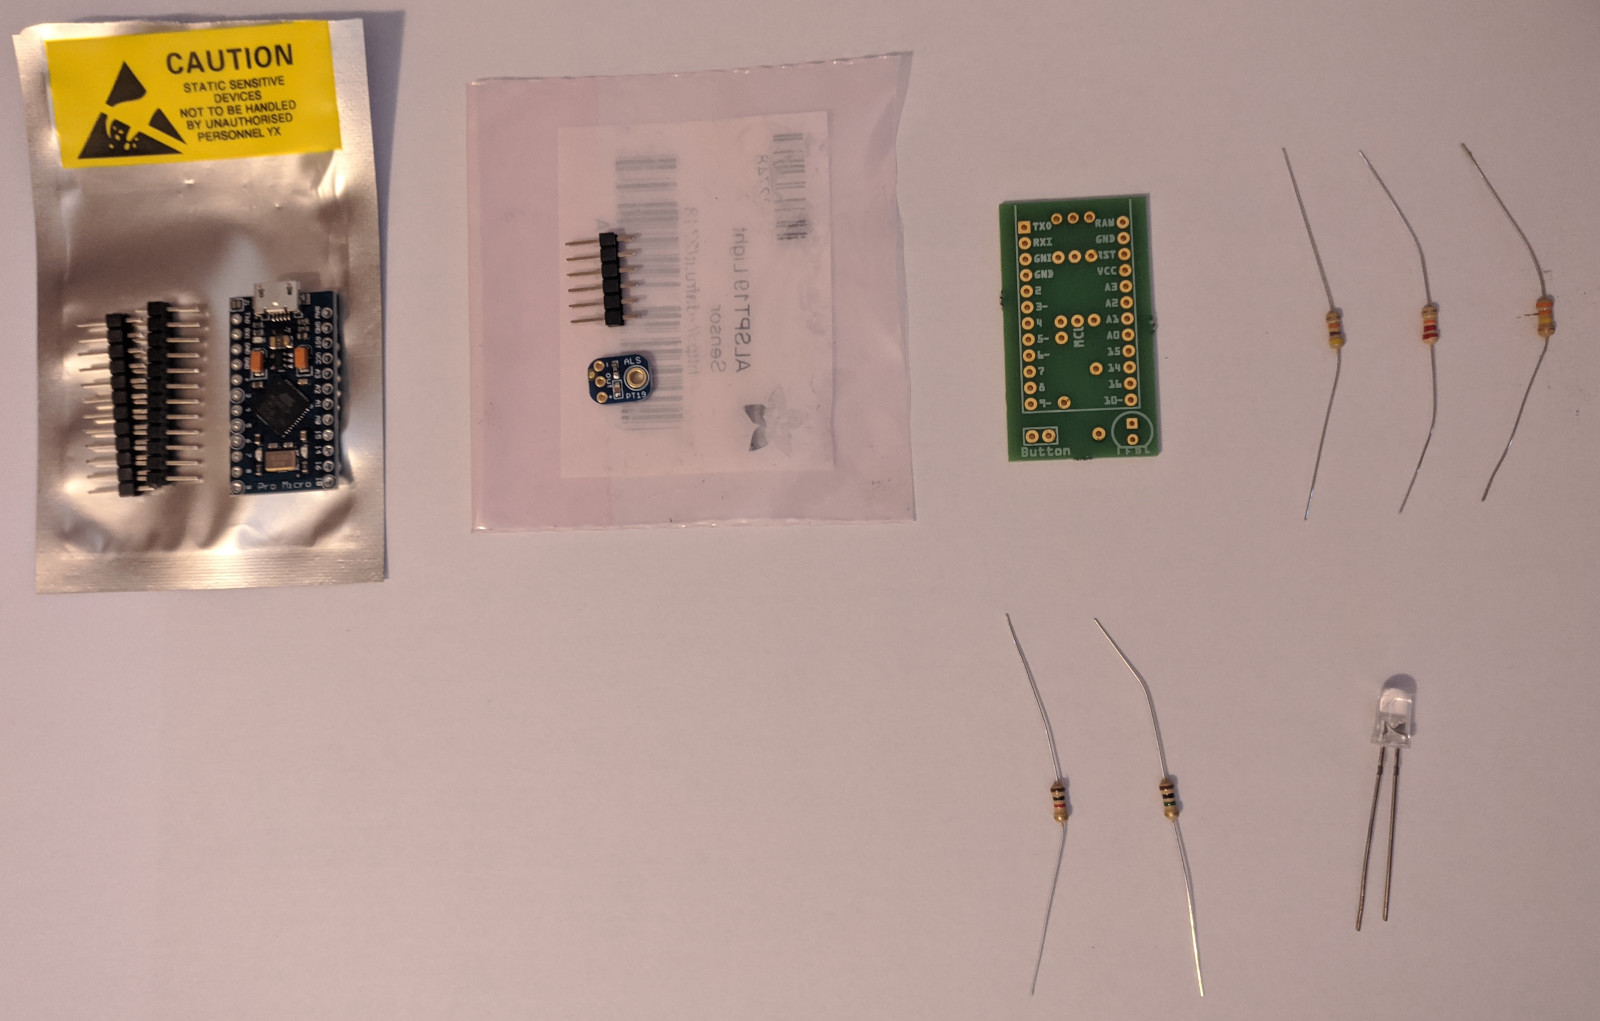
\includegraphics[width=\textwidth]{Chapter03/res/assembly_01.jpg}
	\caption{Materiali necessari per costriuire il dispositivo OpenLDAT}
	\label{fig:assembly_01}
\end{figure}

\begin{figure}[H]
	\centering
	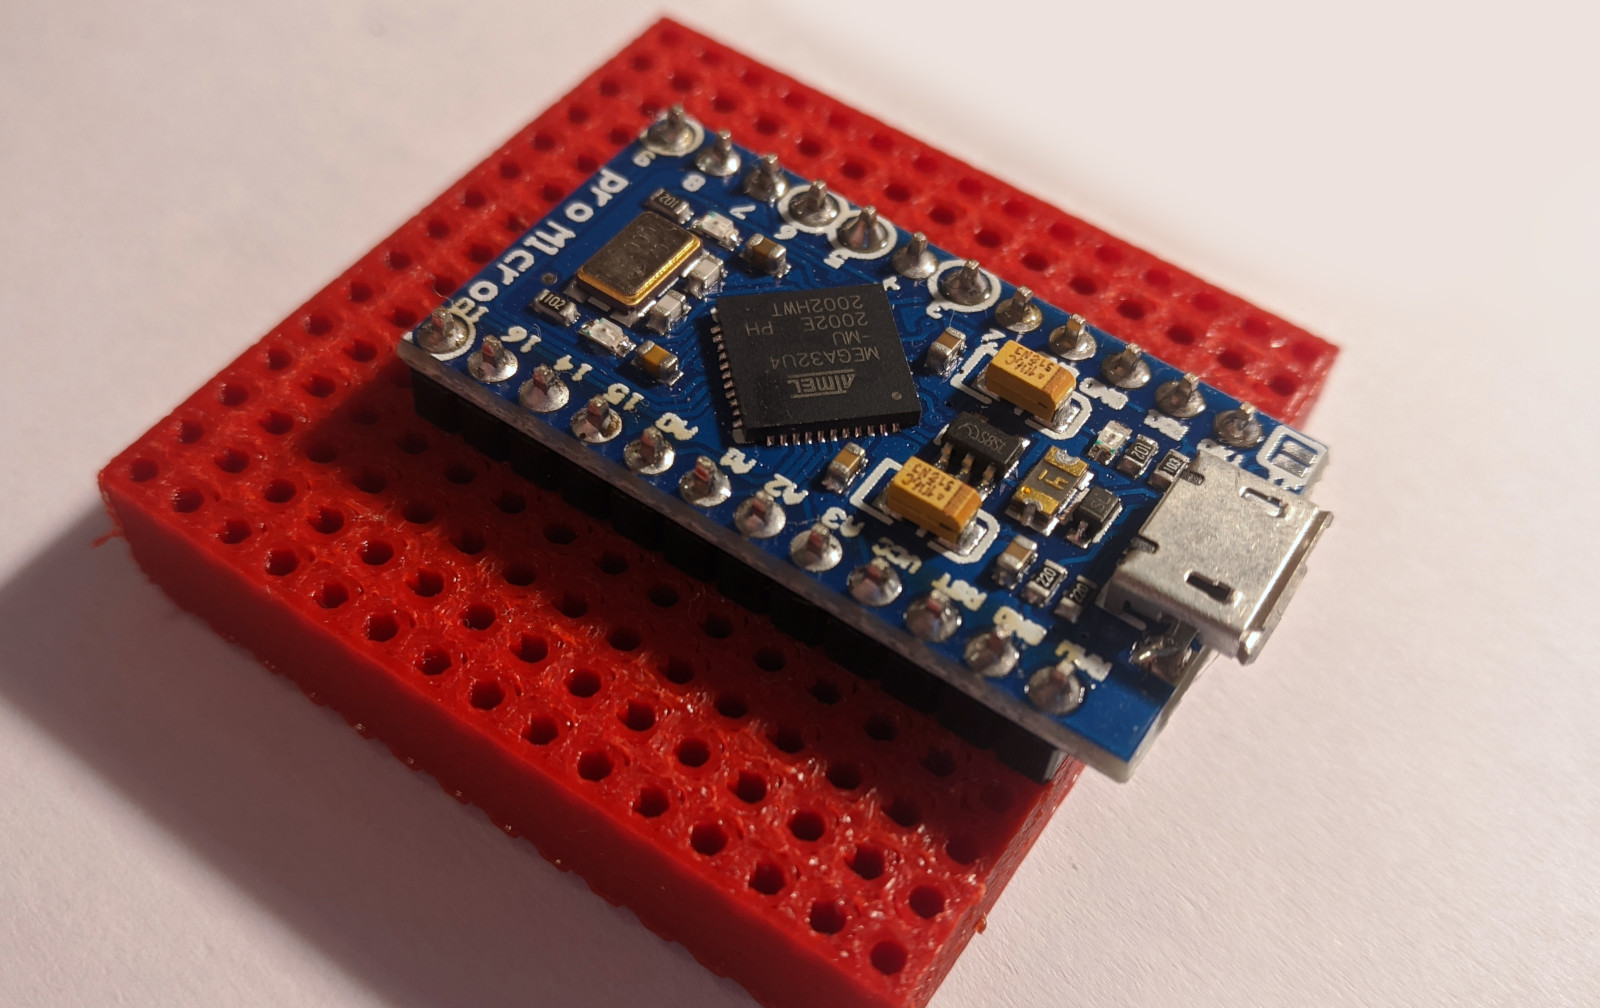
\includegraphics[width=\textwidth]{Chapter03/res/assembly_02.jpg}
	\caption{Preparazione della board Sparkfun Pro Micro}
	\label{fig:assembly_02}
\end{figure}

\begin{figure}[H]
	\centering
	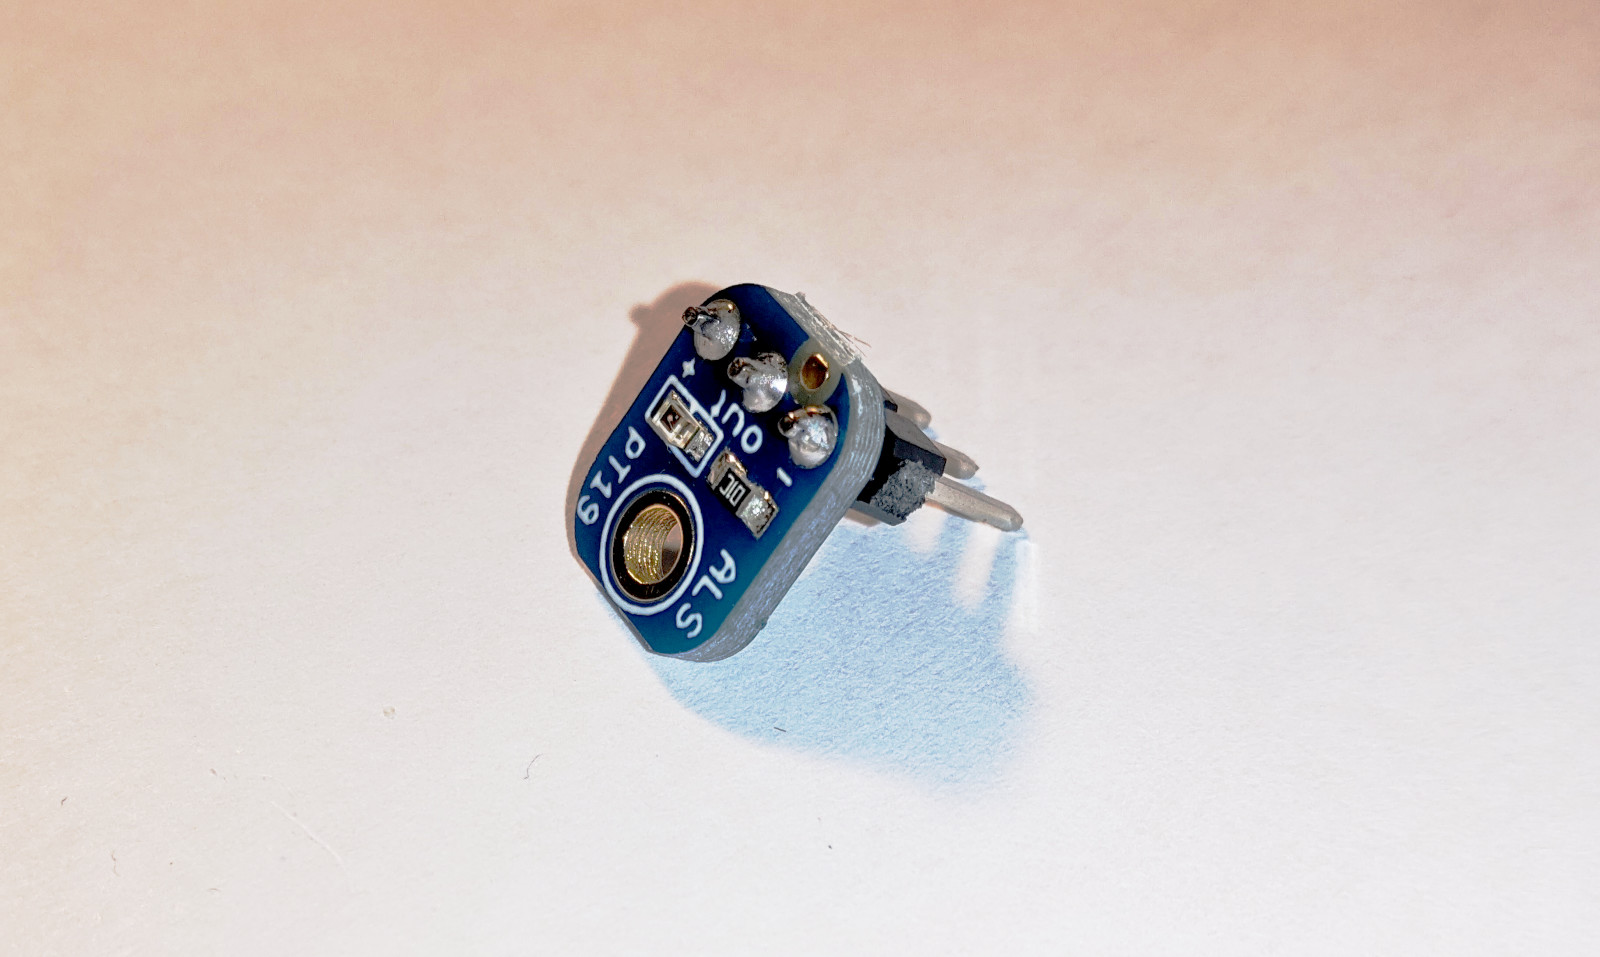
\includegraphics[width=\textwidth]{Chapter03/res/assembly_03.jpg}
	\caption{Preparazione del sensore ALS-PT19}
	\label{fig:assembly_03}
\end{figure}

\begin{figure}[H]
	\centering
	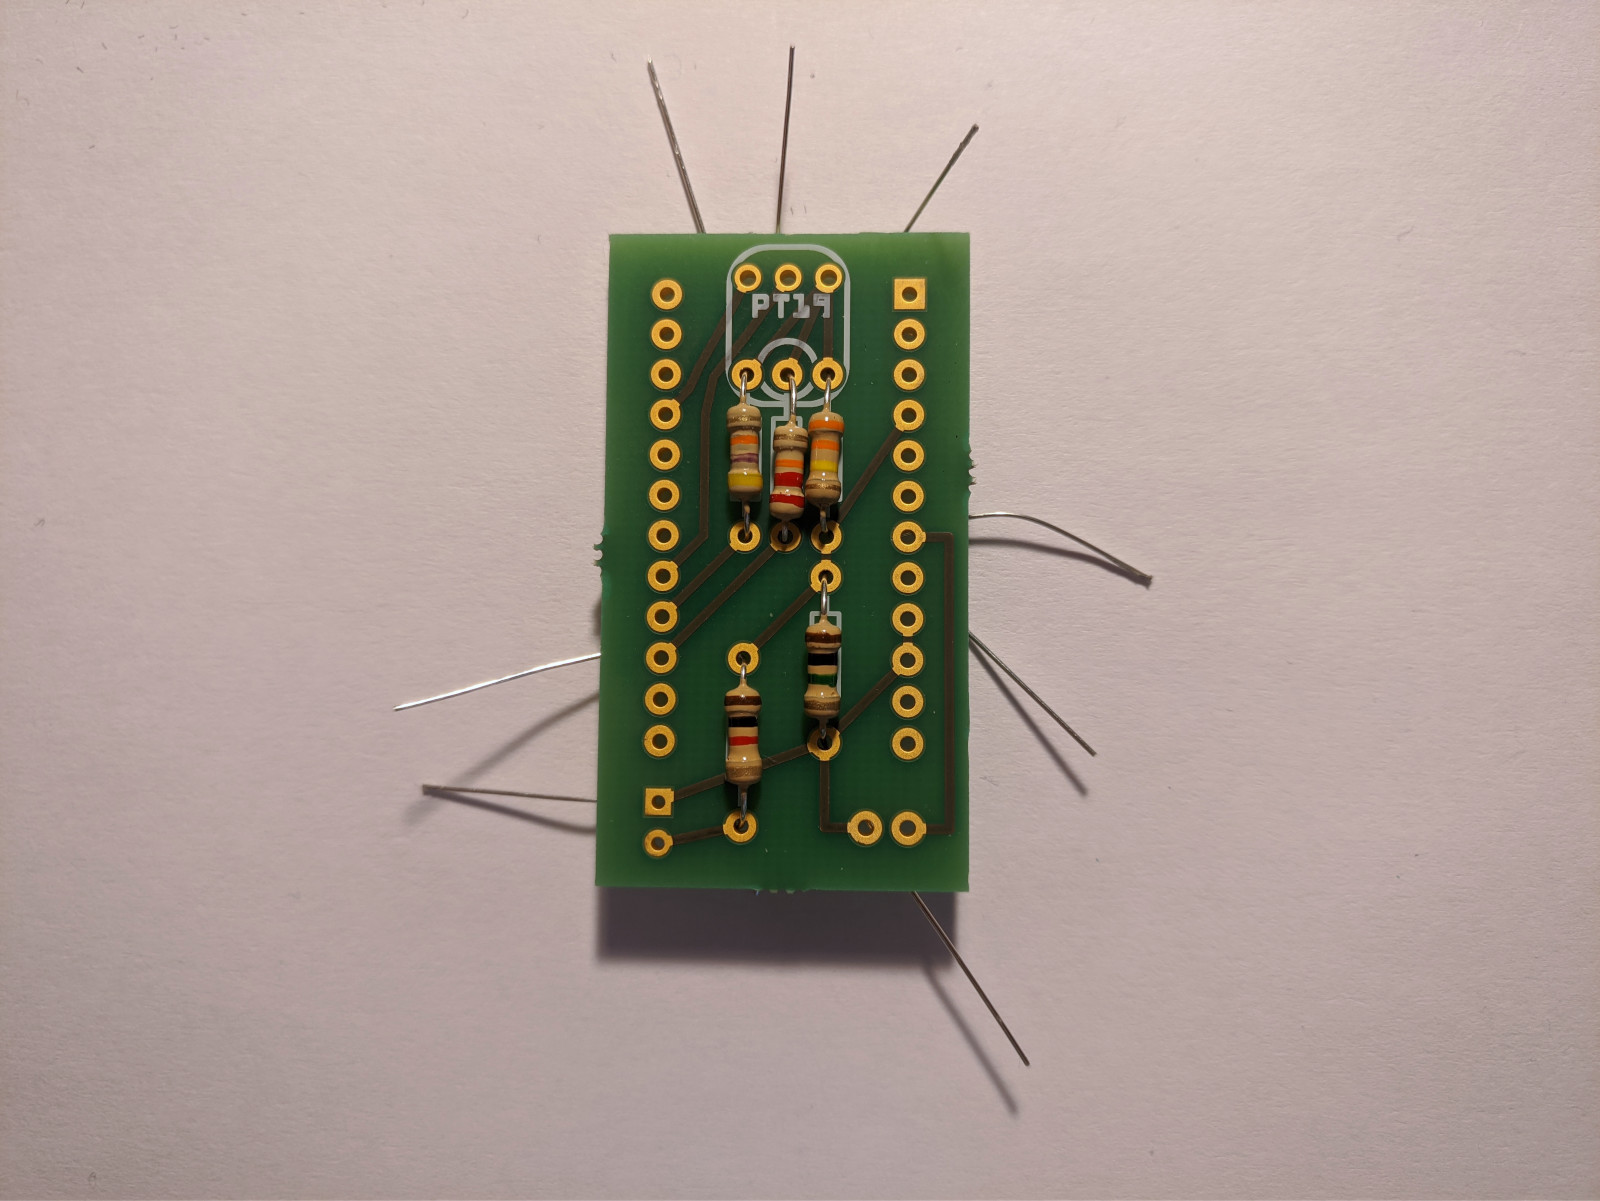
\includegraphics[width=\textwidth]{Chapter03/res/assembly_04.jpg}
	\caption{Posizionamento delle resistenze}
	\label{fig:assembly_04}
\end{figure}

\begin{figure}[H]
	\centering
	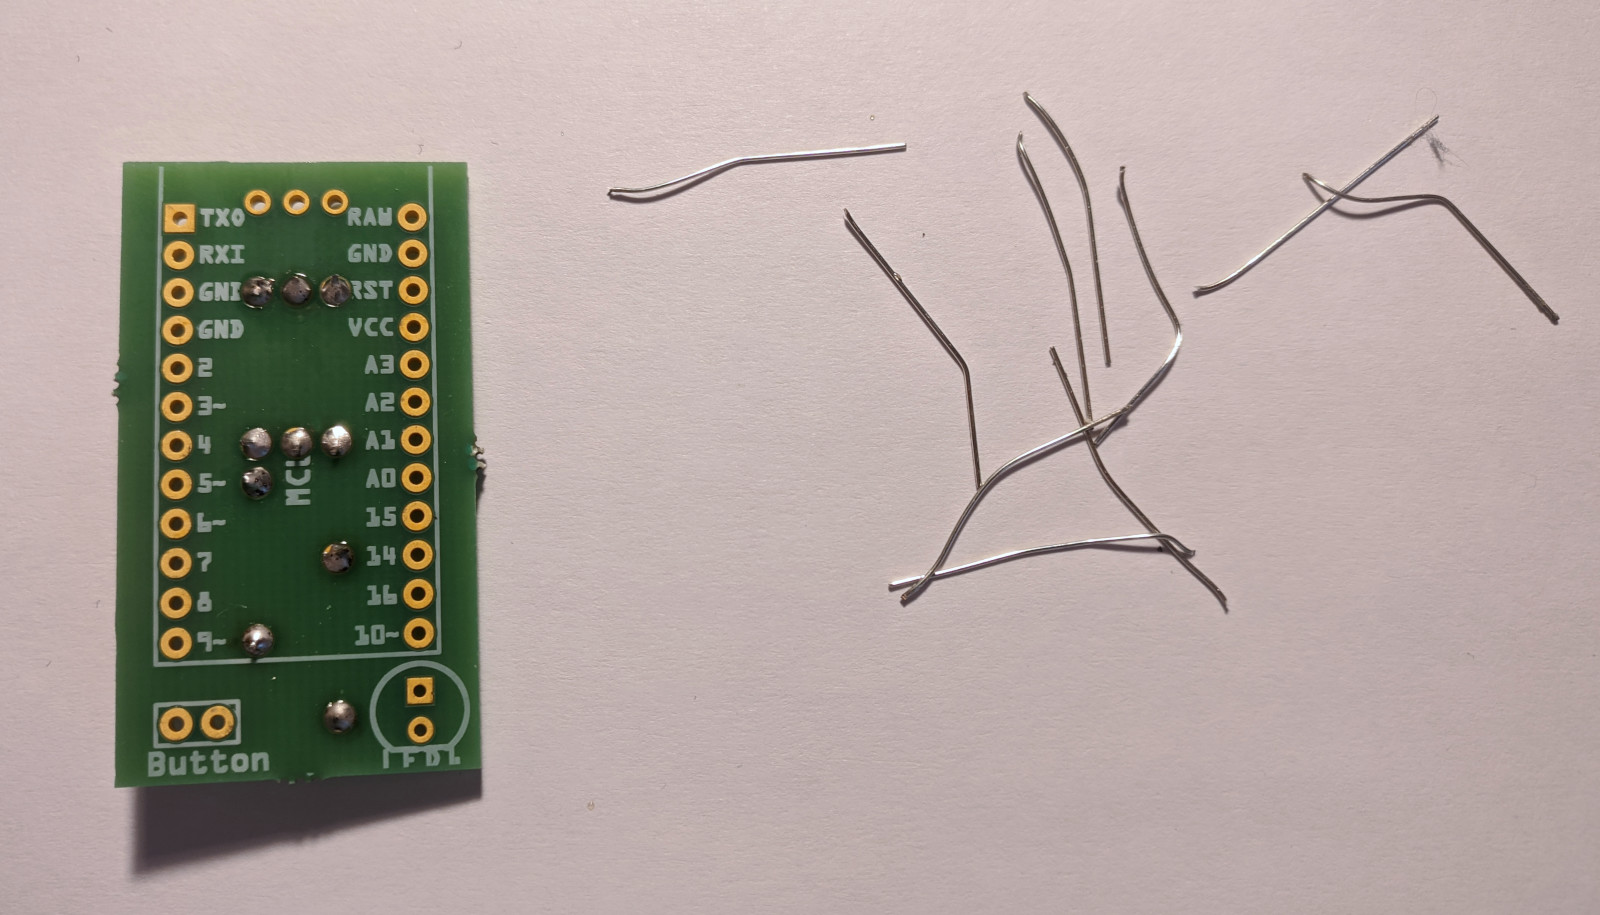
\includegraphics[width=\textwidth]{Chapter03/res/assembly_05.jpg}
	\caption{Resistenze saldate e accorciate}
	\label{fig:assembly_05}
\end{figure}

\begin{figure}[H]
	\centering
	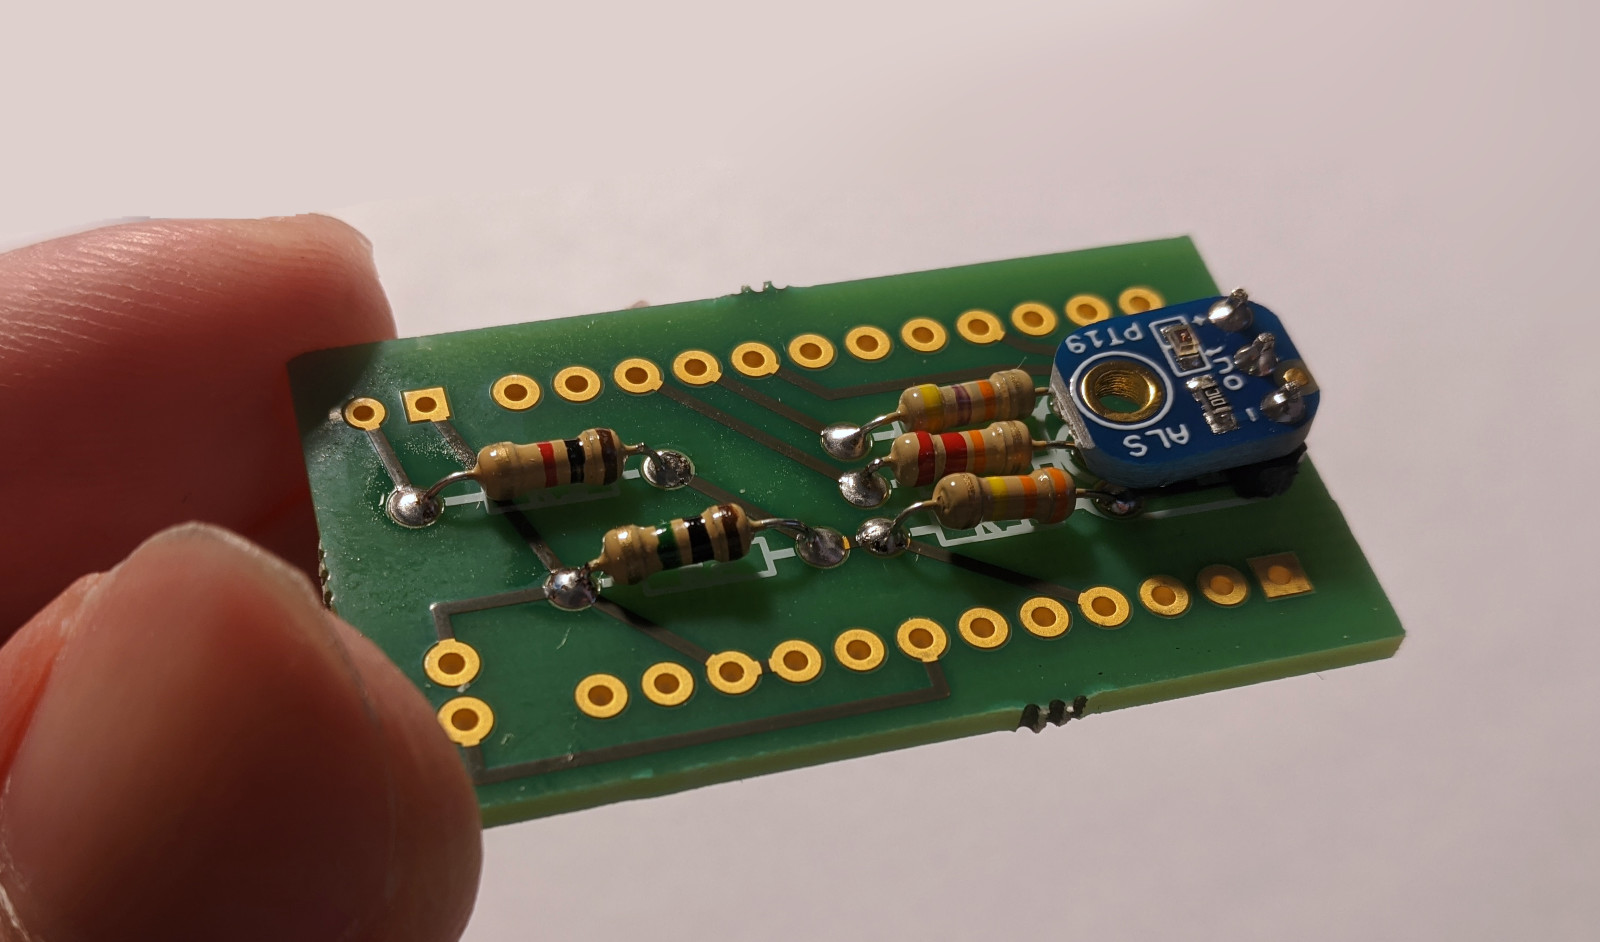
\includegraphics[width=\textwidth]{Chapter03/res/assembly_06.jpg}
	\caption{Posizionamento del sensore ALS-PT19}
	\label{fig:assembly_06}
\end{figure}

\begin{figure}[H]
	\centering
	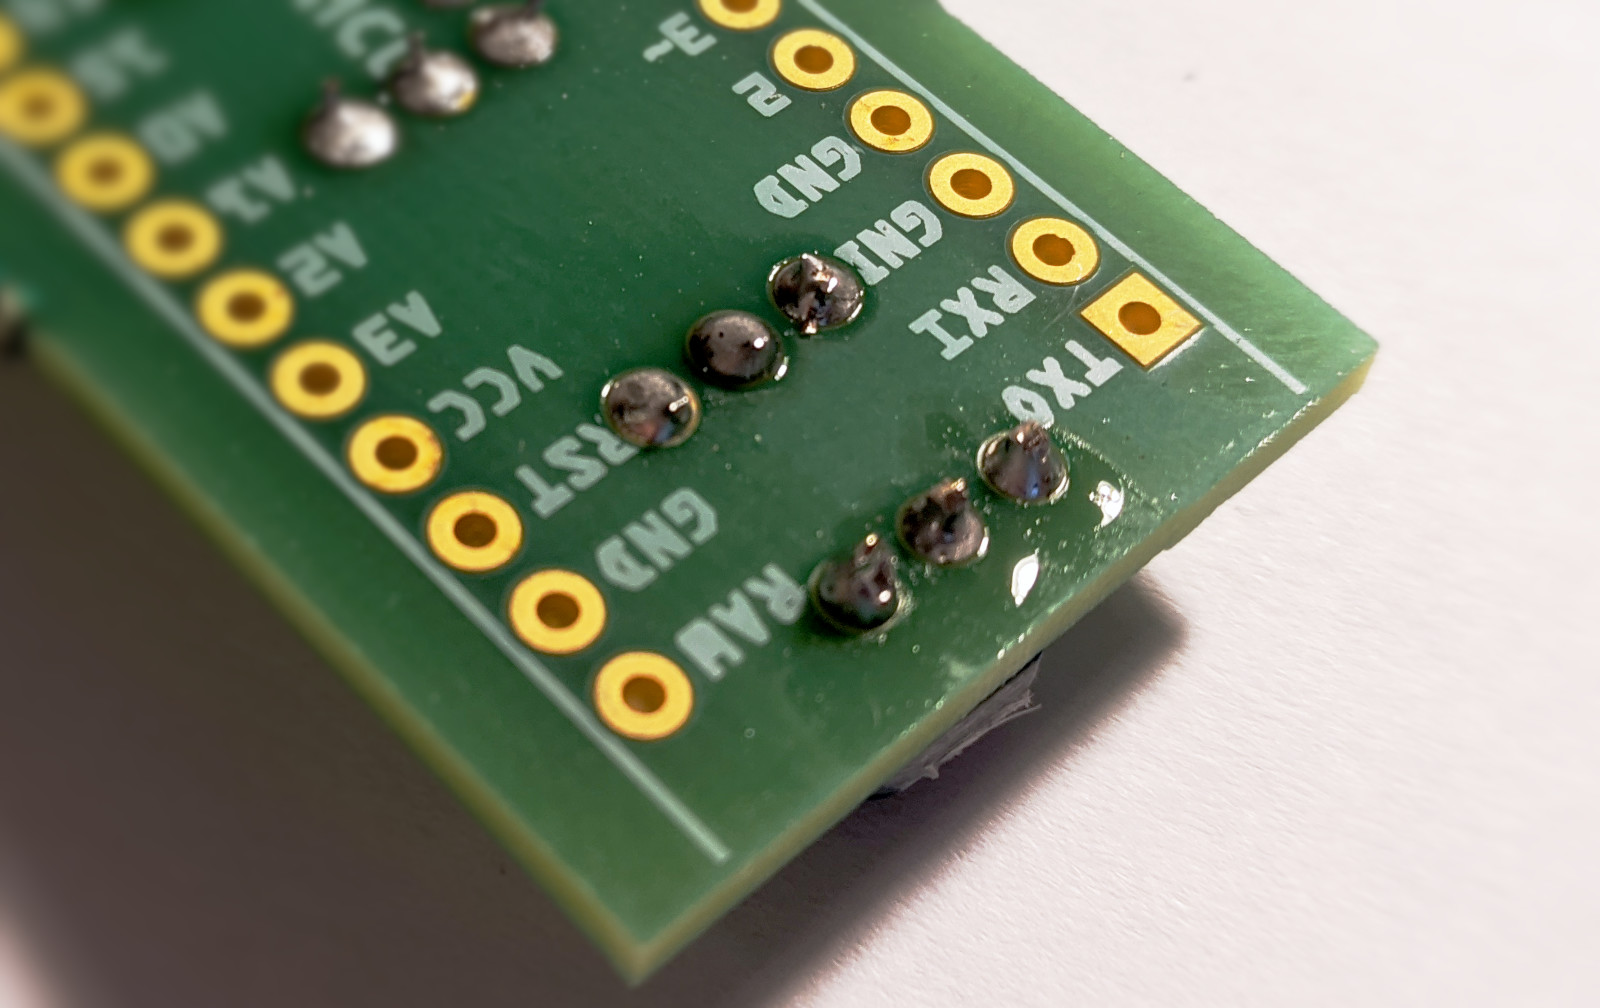
\includegraphics[width=\textwidth]{Chapter03/res/assembly_07.jpg}
	\caption{Sensore saldato e pin accorciati}
	\label{fig:assembly_07}
\end{figure}

\begin{figure}[H]
	\centering
	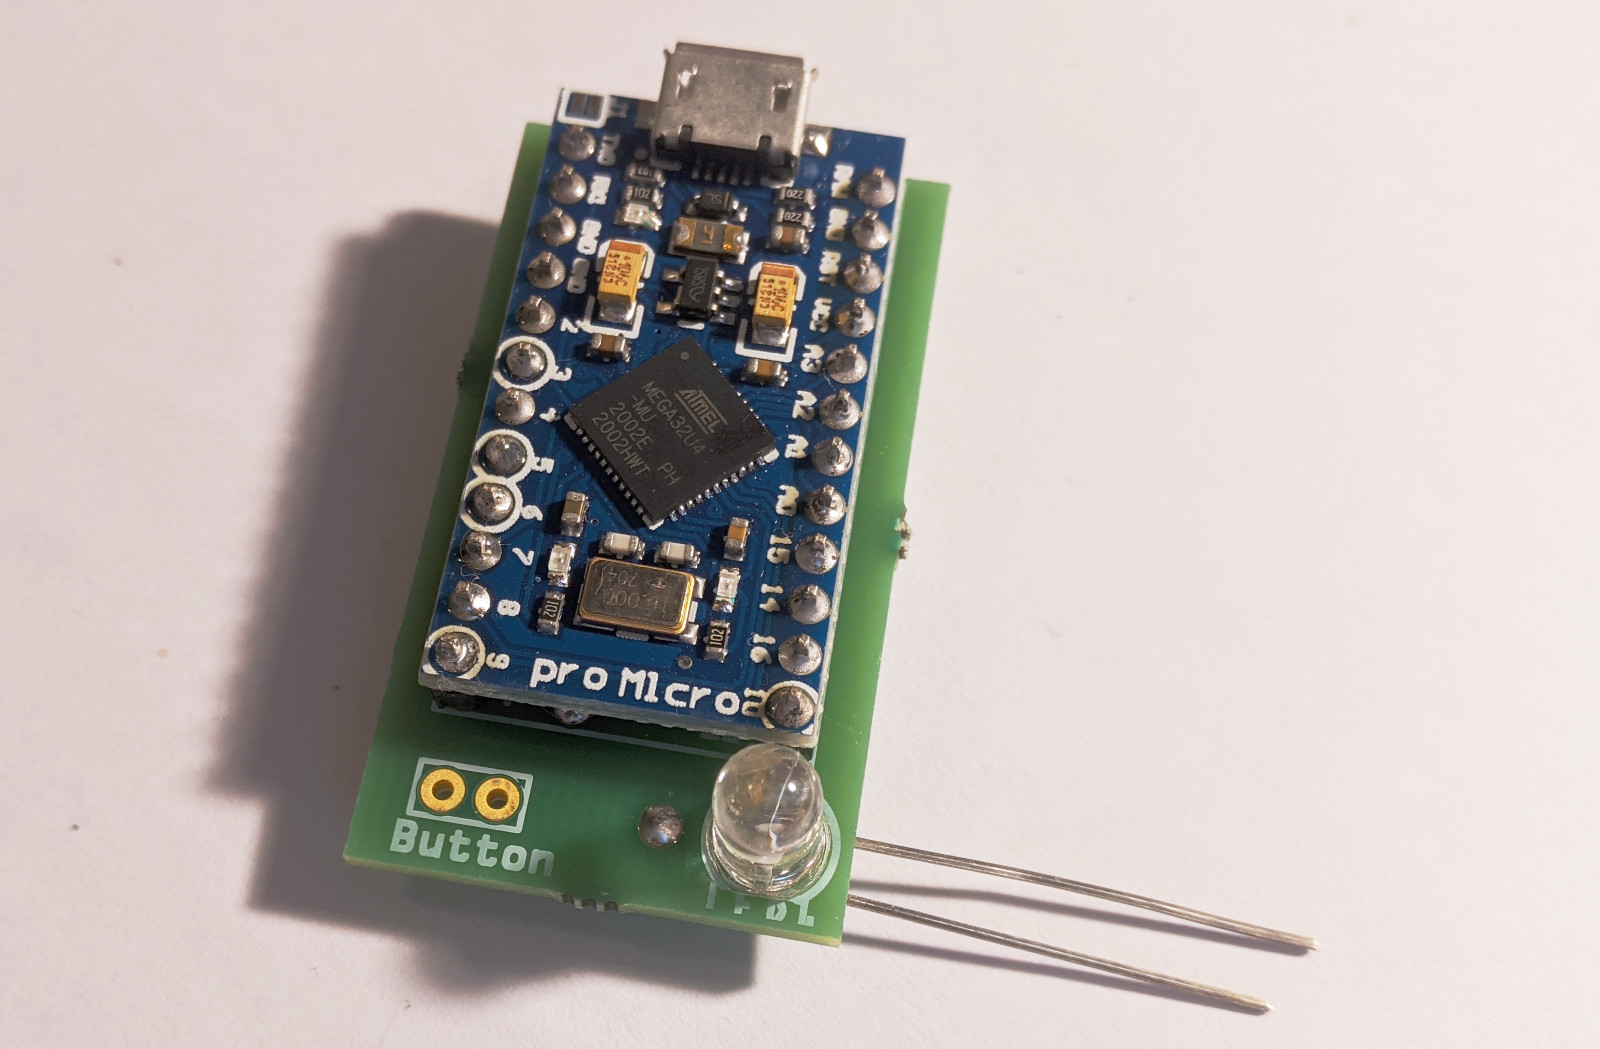
\includegraphics[width=\textwidth]{Chapter03/res/assembly_08.jpg}
	\caption{Posizionamento dello Sparkfun Pro Micro e del LED}
	\label{fig:assembly_08}
\end{figure}

\begin{figure}[H]
	\centering
	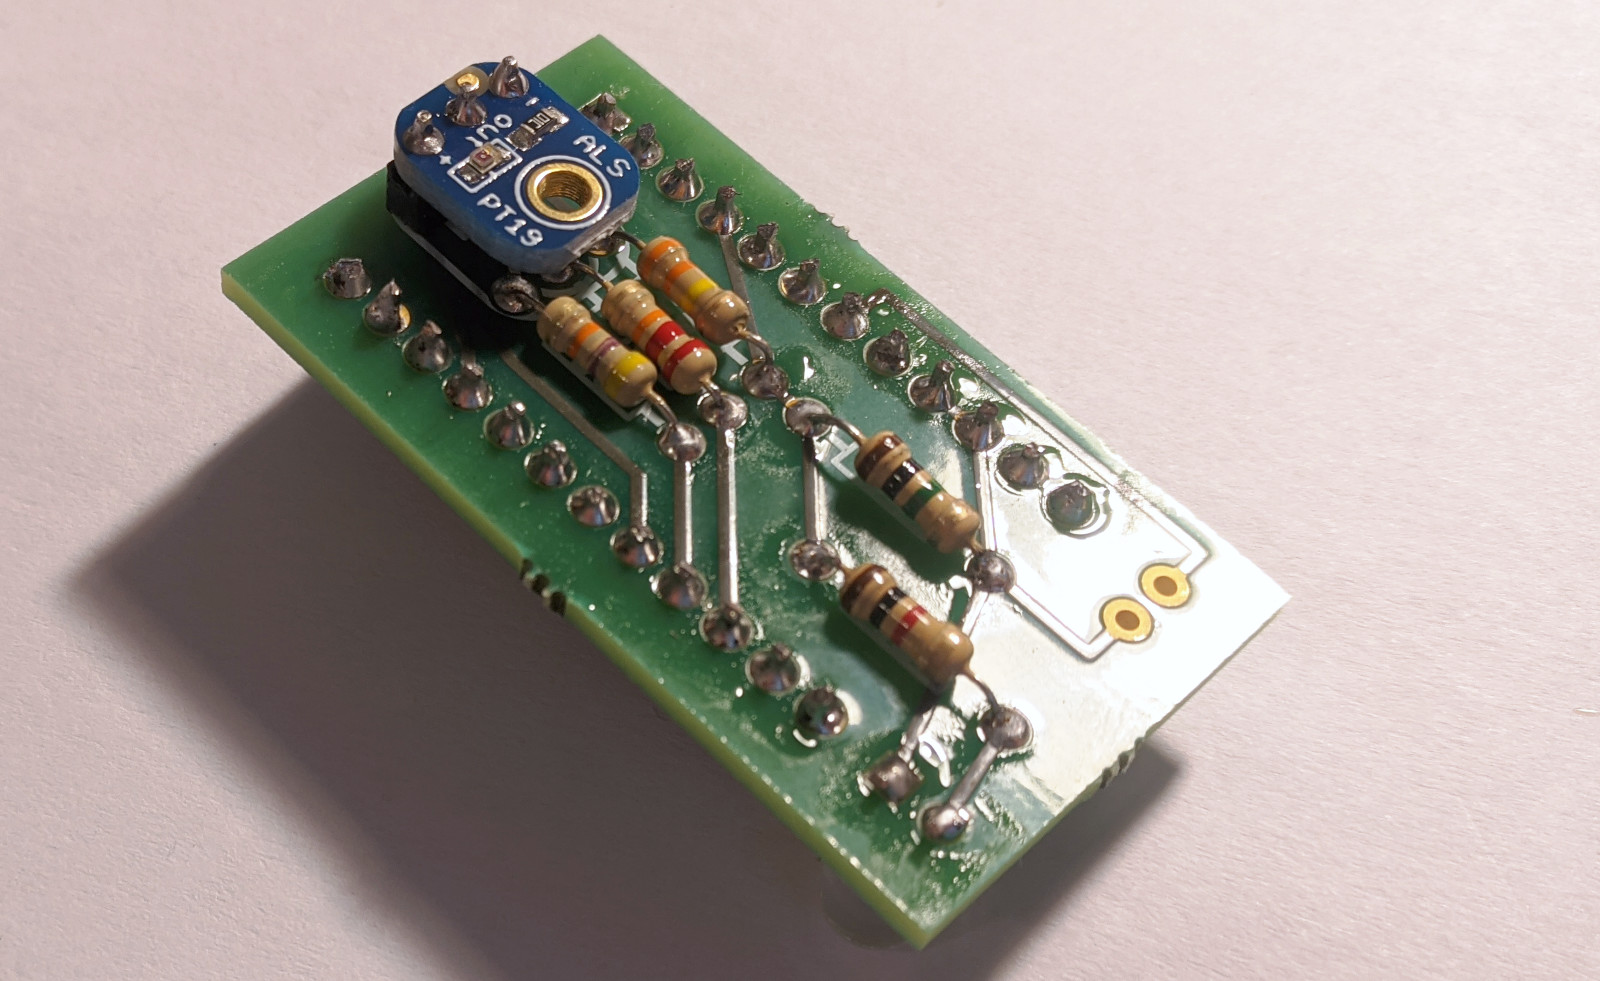
\includegraphics[width=\textwidth]{Chapter03/res/assembly_09.jpg}
	\caption{Board e LED saldati e pin accorciati}
	\label{fig:assembly_09}
\end{figure}

\begin{figure}[H]
	\centering
	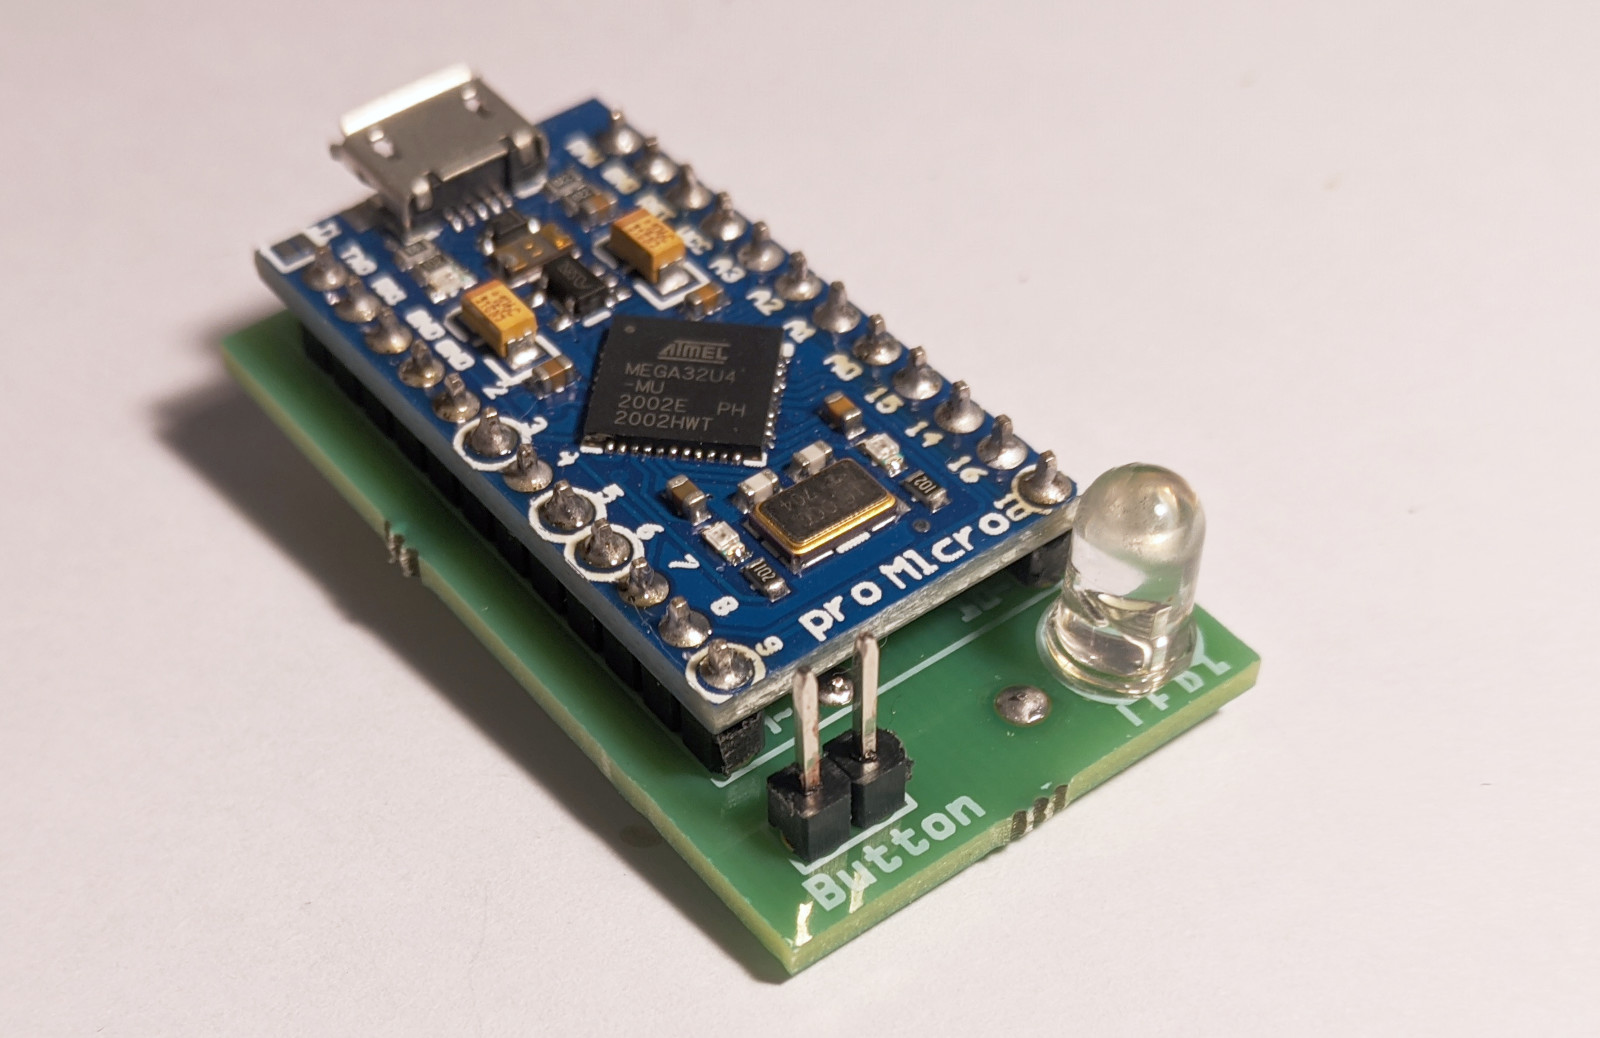
\includegraphics[width=\textwidth]{Chapter03/res/assembly_10.jpg}
	\caption{Assemblaggio del dispositivo completato}
	\label{fig:assembly_10}
\end{figure}

\begin{figure}[H]
	\centering
	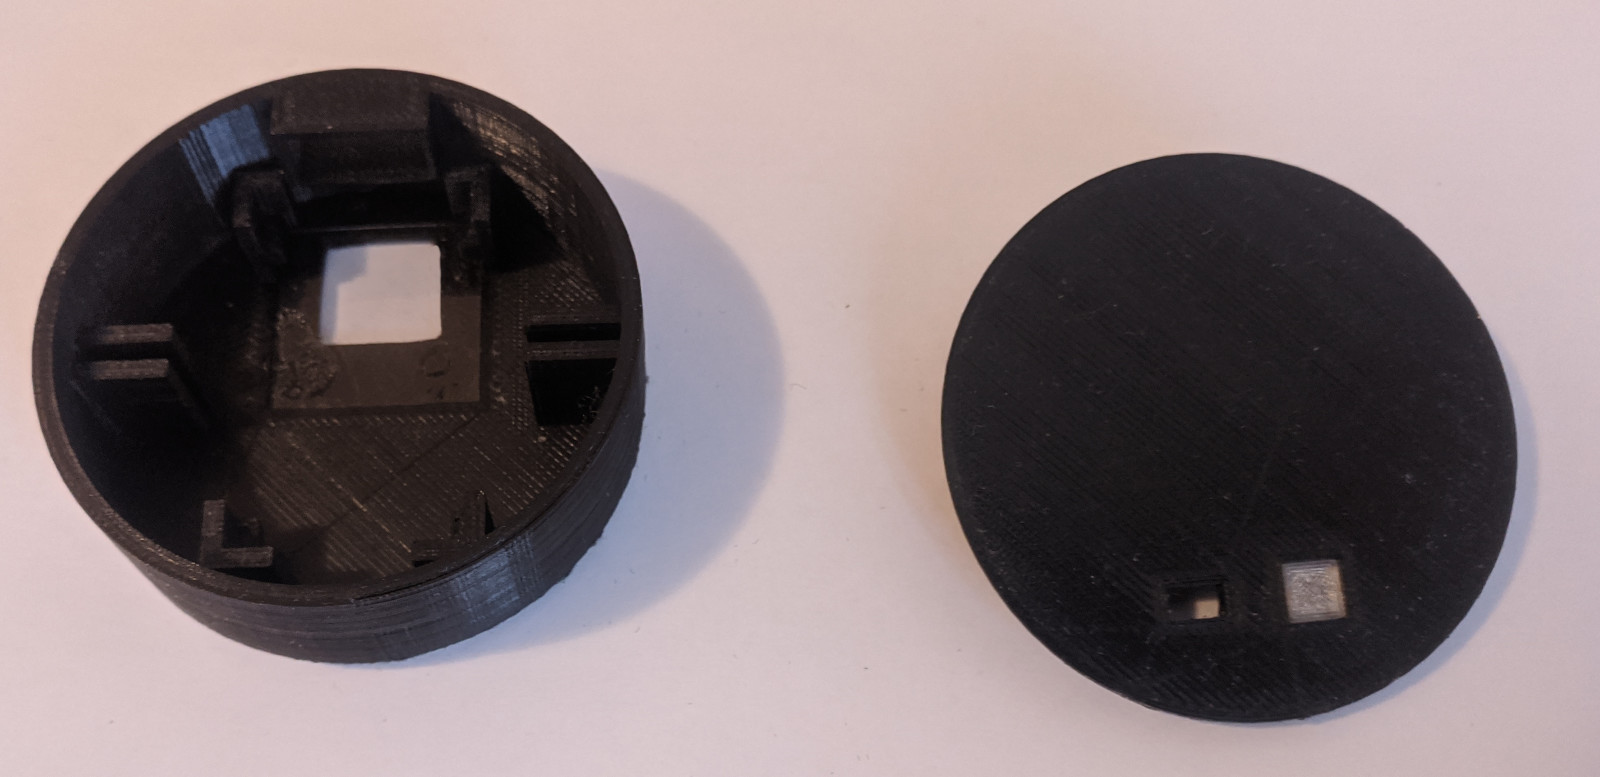
\includegraphics[width=\textwidth]{Chapter03/res/assembly_11.jpg}
	\caption{Parti del case OpenLDAT}
	\label{fig:assembly_11}
\end{figure}

\begin{figure}[H]
	\centering
	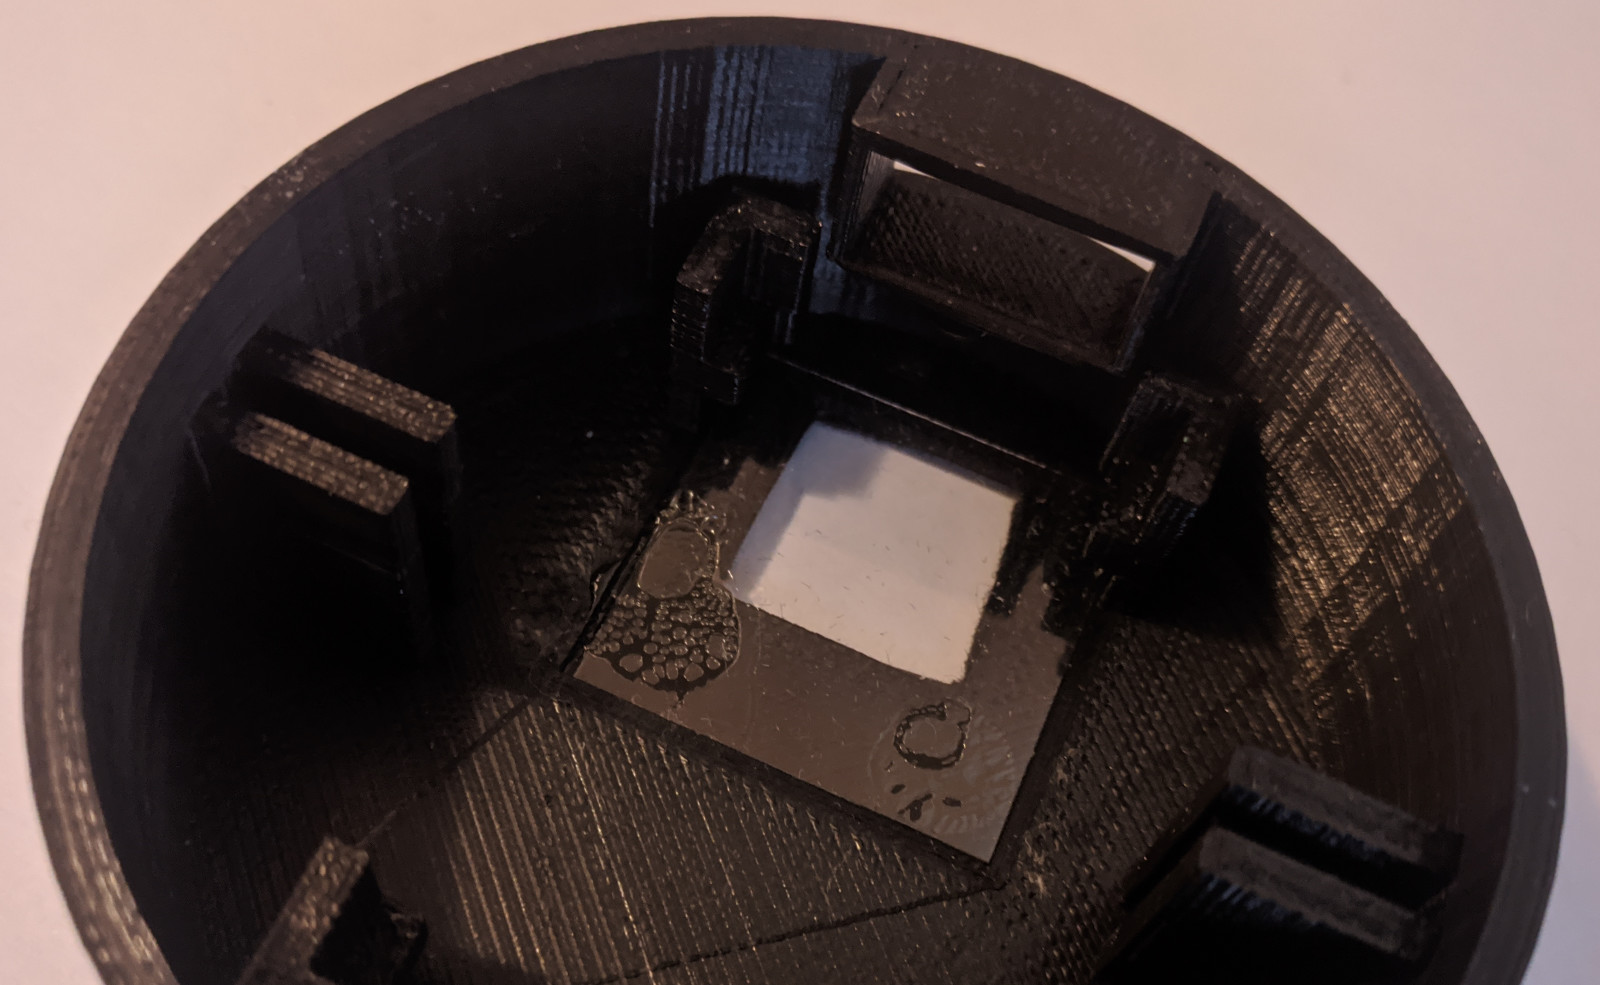
\includegraphics[width=\textwidth]{Chapter03/res/assembly_12.jpg}
	\caption{Posizionamento del vetrino opzionale per proteggere il sensore}
	\label{fig:assembly_12}
\end{figure}

\begin{figure}[H]
	\centering
	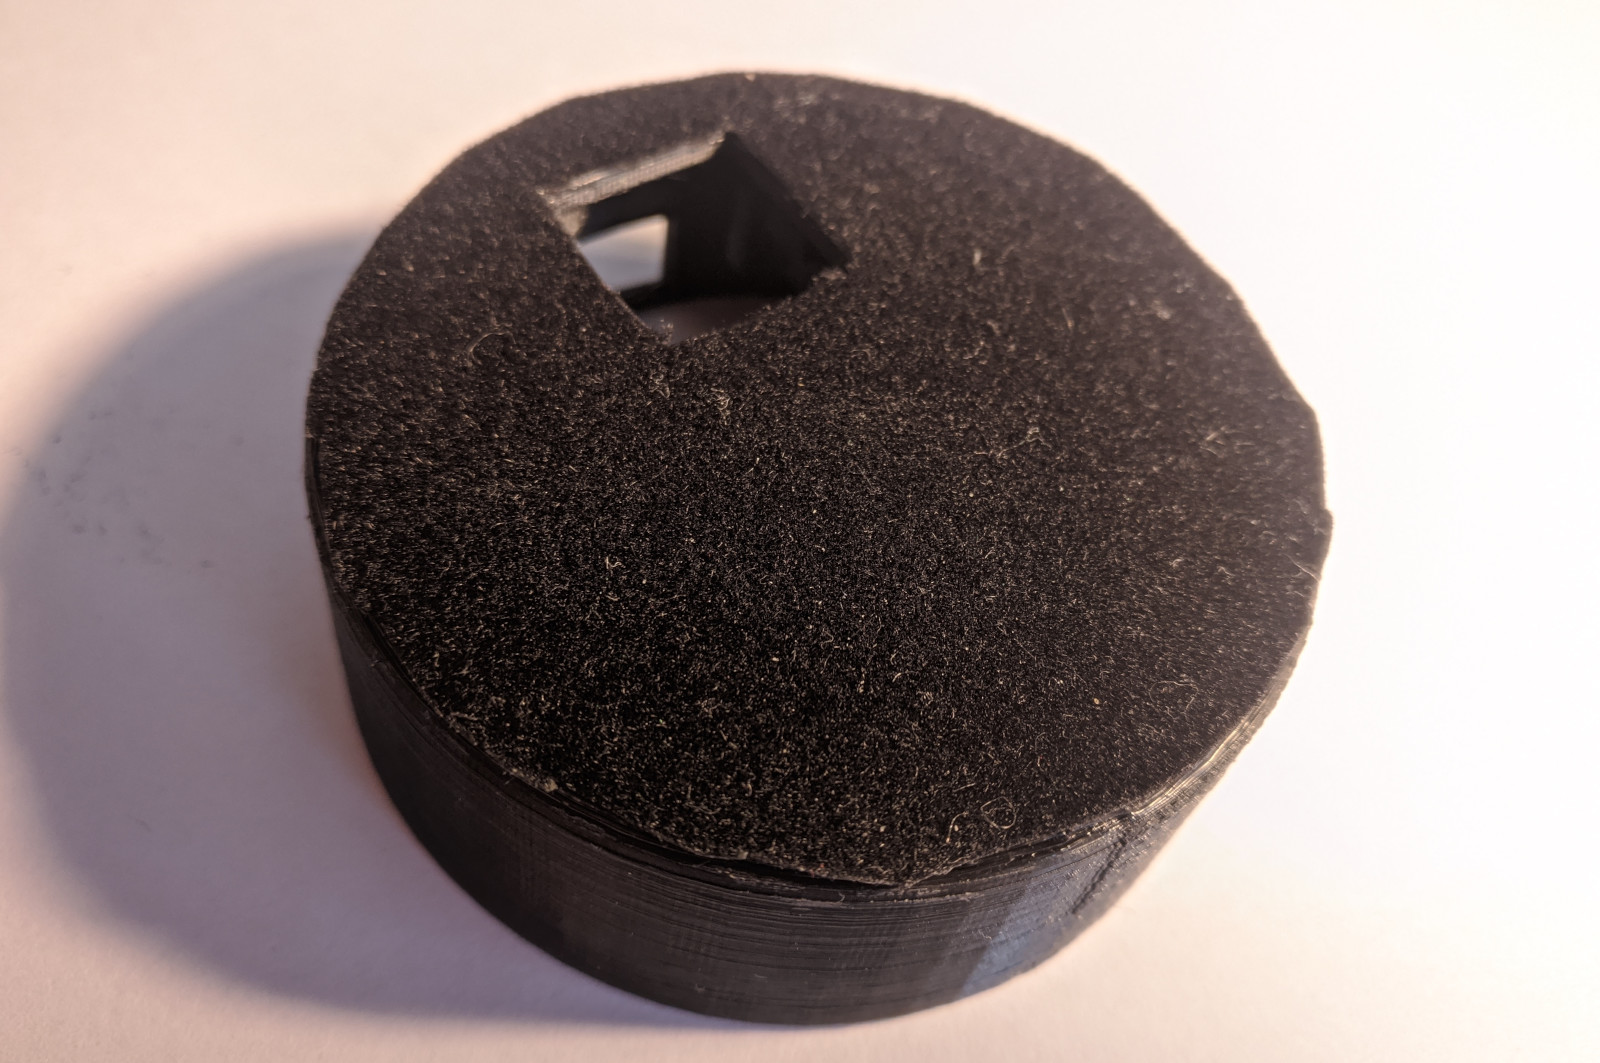
\includegraphics[width=\textwidth]{Chapter03/res/assembly_13.jpg}
	\caption{Carta adesiva vellutata per proteggere il display da graffi accidentali}
	\label{fig:assembly_13}
\end{figure}

\begin{figure}[H]
	\centering
	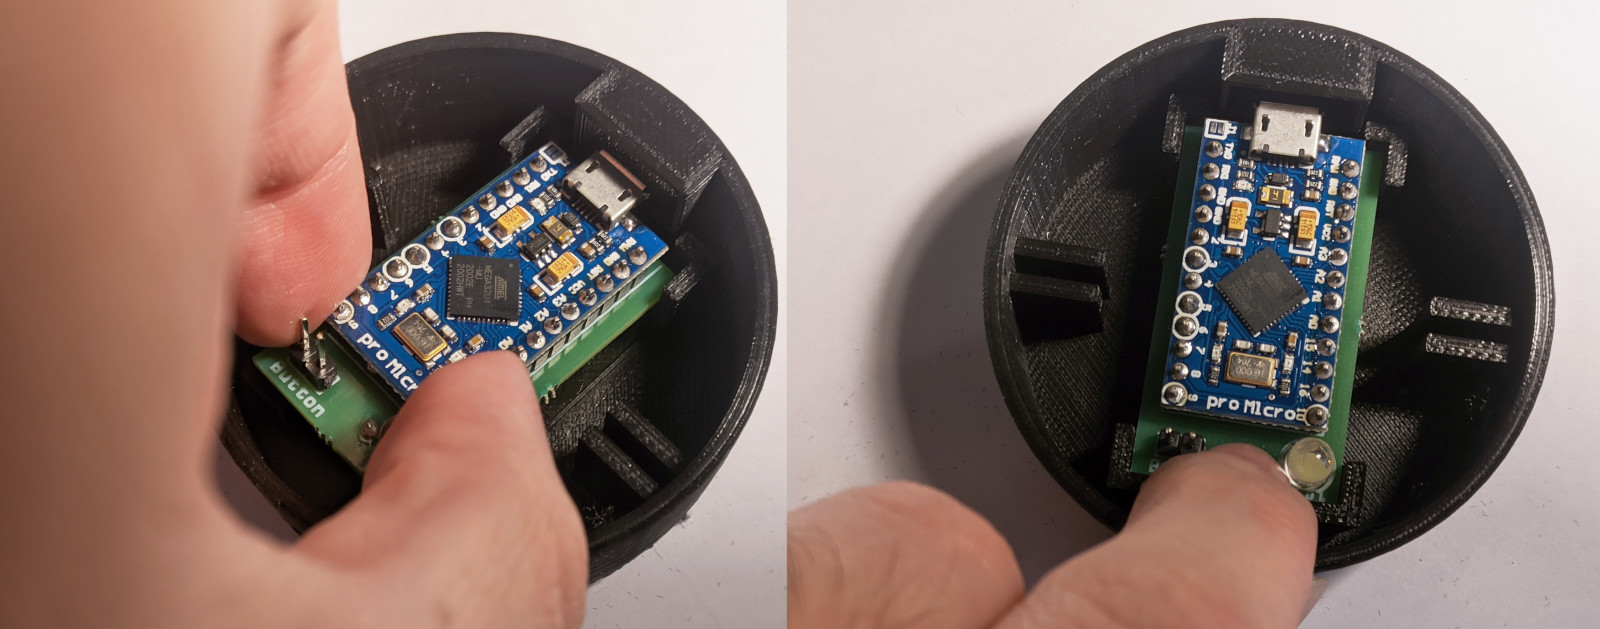
\includegraphics[width=\textwidth]{Chapter03/res/assembly_14.jpg}
	\caption{Inserimento del PCB nel case}
	\label{fig:assembly_14}
\end{figure}

\begin{figure}[H]
	\centering
	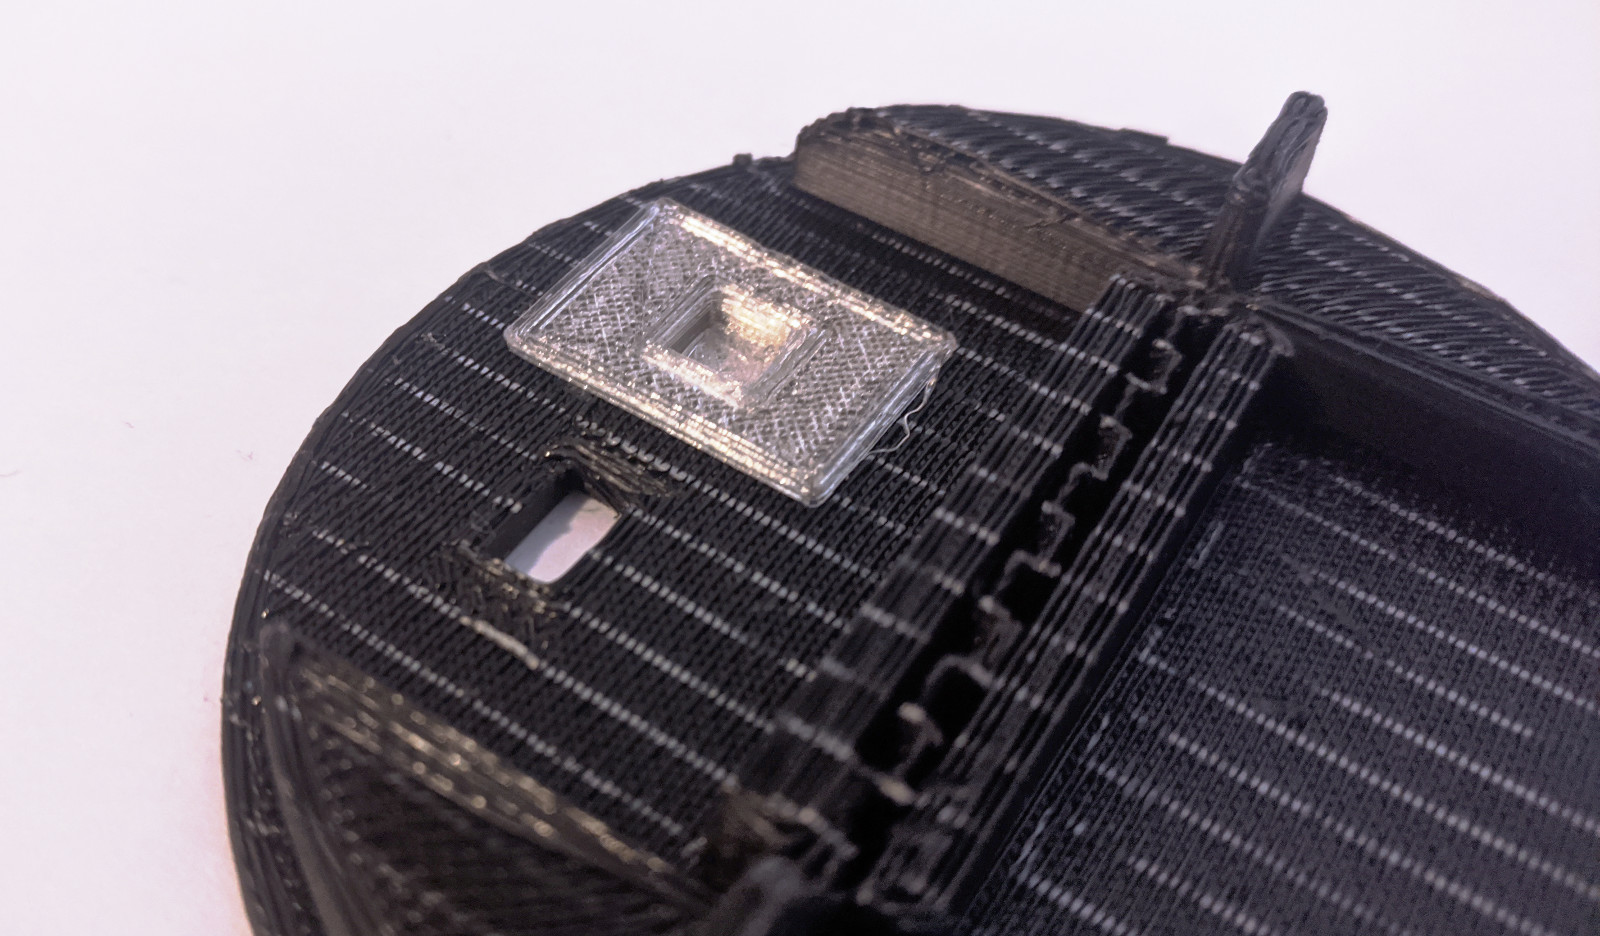
\includegraphics[width=\textwidth]{Chapter03/res/assembly_16.jpg}
	\caption{Diffusore per il LED montato sul coperchio}
	\label{fig:assembly_16}
\end{figure}

\begin{figure}[H]
	\centering
	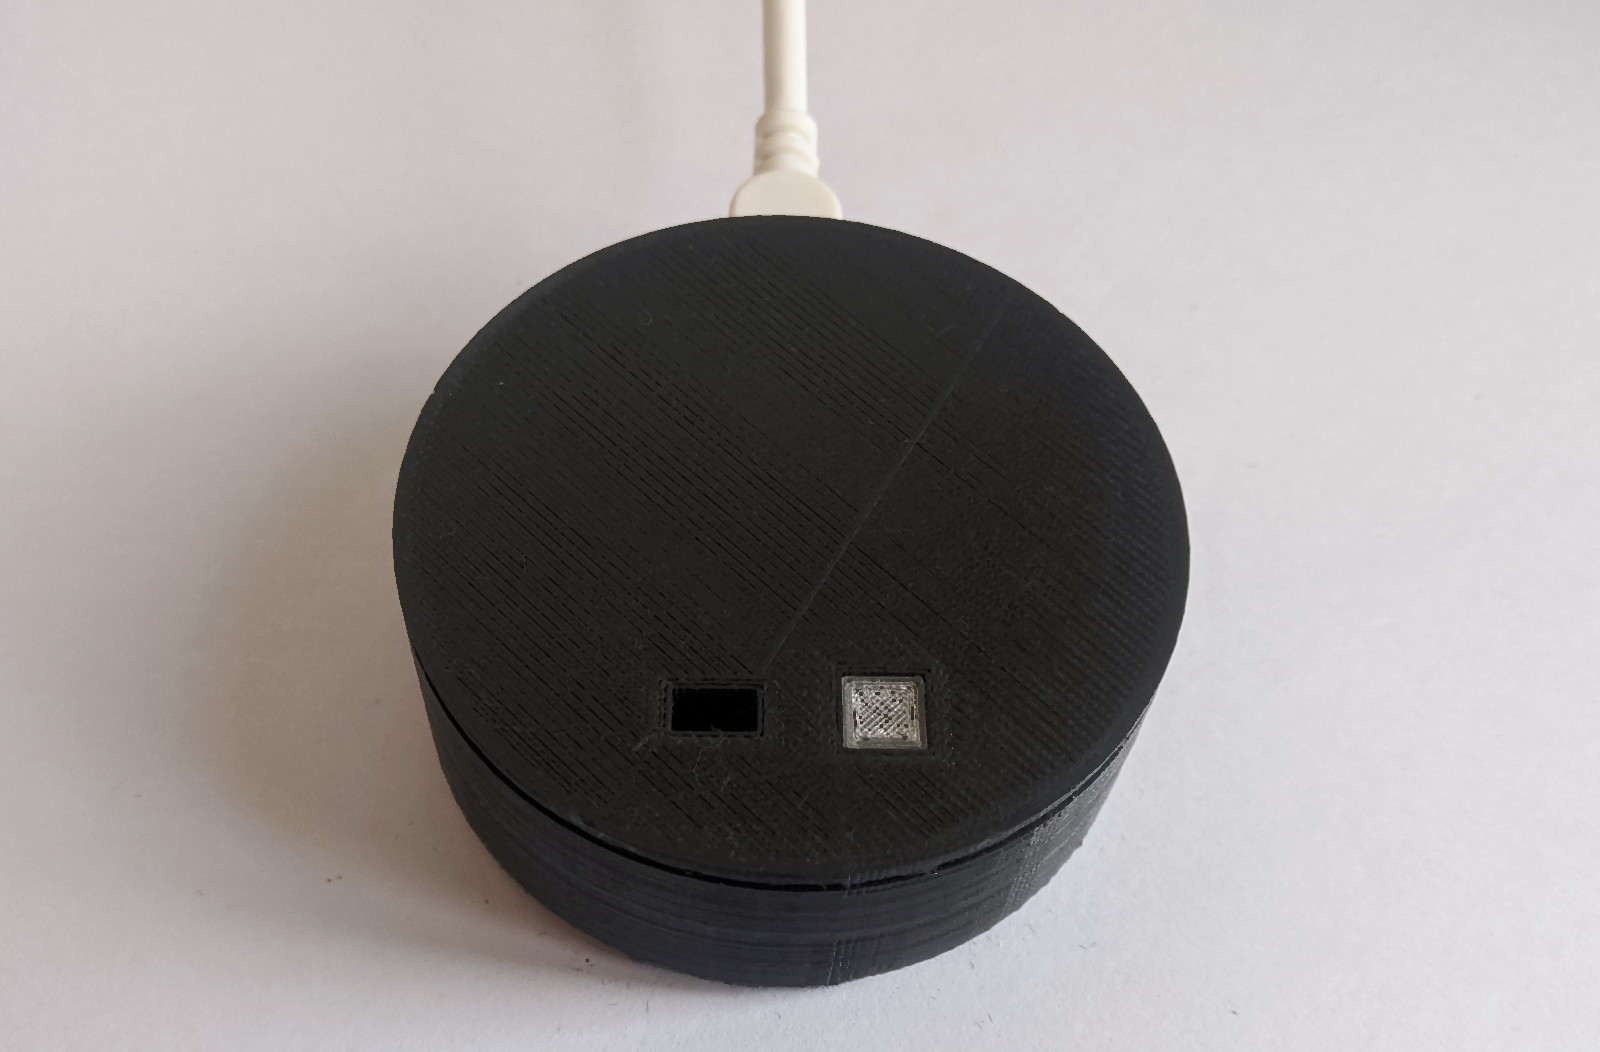
\includegraphics[width=\textwidth]{Chapter03/res/assembly_15.jpg}
	\caption{Dispositivo OpenLDAT assemblato}
	\label{fig:assembly_15}
\end{figure}

\subsection{Flashing}
Il dispositivo OpenLDAT è inutile senza il suo firmware, per cui va flashato prima di utilizzarlo. Vengono forniti due metodi per caricare il firmware:
\begin{itemize}
	\item \textbf{Script automatico}: assieme al firmware viene fornito uno script che flasha il dispositivo con un firmware precompilato e testato. Questa è la soluzione consigliata per chi vuole solo utilizzare OpenLDAT e non sviluppare. Al momento lo script è disponibile per GNU/Linux e Windows
	\item \textbf{Usando Arduino IDE}: il progetto del firmware può essere caricato in Arduino IDE e flashato da lì. Questa è la soluzione ideale per chi vuole sviluppare versioni modificate del firmware, ma richiede che l'IDE venga configurata opportunamente e introduce alcune complicazioni
\end{itemize}

Le due sezioni successive spiegano passo-passo come flashare il dispositivo con questi due metodi.

\subsubsection{Flashing con lo script automatico (GNU/Linux)}
All'interno della cartella del firmware è presente una cartella chiamata \texttt{Prebuilt}, all'interno della quale è presente il firmware precompilato e lo script \texttt{flash.sh}.

\paragraph{Passo 1} Installare python e avrdude dal package manager della propria distribuzione. Supponendo di essere su Ubuntu, questo comando installa i due package necessari per il flashing:
\begin{verbatim}
	sudo apt install python3 avrdude
\end{verbatim}

\paragraph{Passo 2} Aprire un terminale all'interno della cartella \texttt{Prebuilt}, collegare il dispositivo da flashare, e prendere nota del nome che viene assegnato alla porta seriale del dispositivo. Questo comando permette di elencare le porte seriali attualmente assegnate:
\begin{verbatim}
	ls -l /dev/serial/by-id
\end{verbatim}

Nell'esempio in figura \ref{fig:flashing_01}, al dispositivo viene assegnato il nome \texttt{ttyACM0}.

\paragraph{Passo 3} Flashare il dispositivo eseguendo il seguente comando, sostituendo a \texttt{device} il nome della porta seriale determinato nel passo precedente:
\begin{verbatim}
	sudo ./flash.sh /dev/device
\end{verbatim}

Lo script richiederà alcuni secondi per essere eseguito, durante i quali produce un output dettagliato delle attività. Se la procedura viene completata correttamente, al termine viene visualizzato il messaggio "Successs! You now have an OpenLDAT device" come in figura \ref{fig:flashing_02}.\\
Se si verificano degli errori durante la procedura, i dettagli verranno mostrati per consentire di capire il problema.

Attenzione: è raro ma possibile che il nome della porta seriale assegnata al dispositivo cambi durante l'esecuzione dello script facendolo fallire. Se dovesse succedere, si può riprovare con un'altra porta USB o un altro PC, oppure utilizzando Arduino IDE.

\begin{figure}[H]
	\centering
	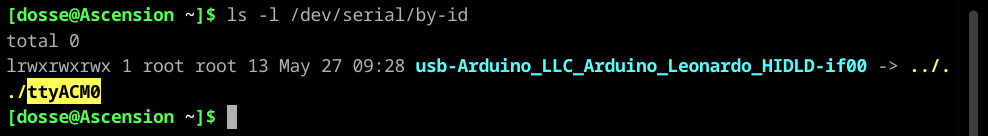
\includegraphics[width=\textwidth]{Chapter03/res/flashing_01.png}
	\caption{Esempio di elenco dei dispositivi seriali}
	\label{fig:flashing_01}
\end{figure}

\begin{figure}[H]
	\centering
	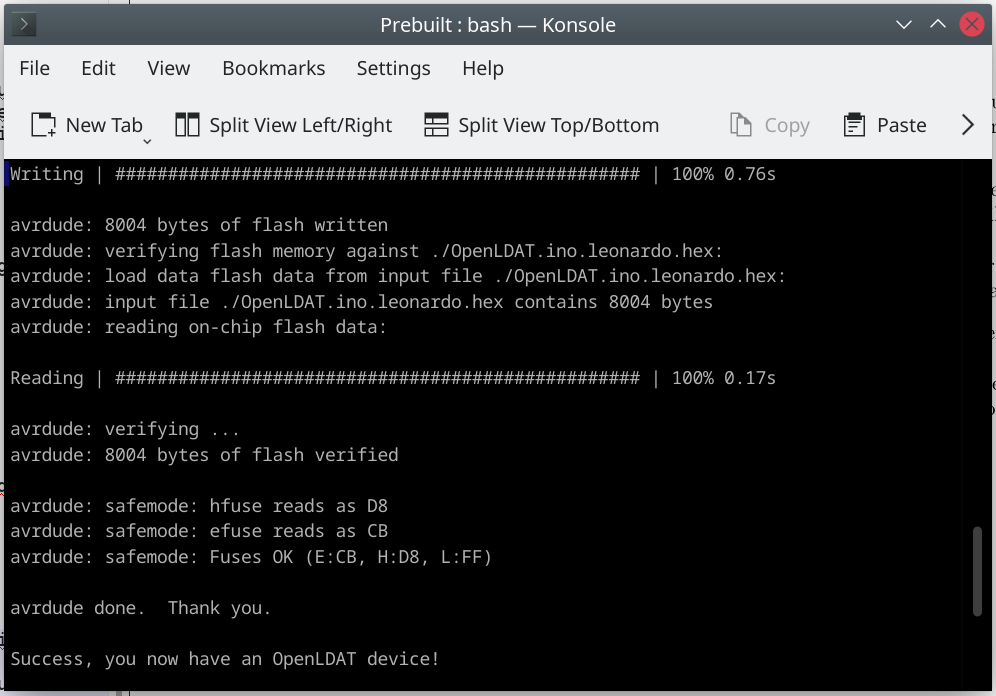
\includegraphics[width=\textwidth]{Chapter03/res/flashing_02.png}
	\caption{Output dello script automatico}
	\label{fig:flashing_02}
\end{figure}

\subsubsection{Flashing con lo script automatico (Windows)}
All'interno della cartella del firmware è presente una cartella chiamata \texttt{Prebuilt}, all'interno della quale è presente il firmware precompilato e lo script \texttt{flash.bat} per Windows.

\paragraph{Passo 1} Installare Arduino IDE utilizzando l'installatore sul sito web\footnote{\href{https://www.arduino.cc/en/software}{https://www.arduino.cc/en/software}}, lasciando i file nel loro percorso di default, e assicurandosi di installare anche i driver di Arduino.

\paragraph{Passo 2} Collegare il dispositivo da flashare, entrare nella cartella \texttt{Prebuilt} e fare doppio click su flash.bat per visualizzare l'elenco di porte COM, come in figura figura \ref{fig:flashing_07}. Prendere nota della porta del dispositivo da flashare, nell'esempio è \texttt{COM6}.

\paragraph{Passo 3} Aprire un terminale all'interno della cartella Prebuilt ed eseguire il seguente comando, sostituendo a \texttt{COM6} la porta del dispositivo da flashare determinata nel passo precedente:
\begin{verbatim}
	.\flash.bat COM6
\end{verbatim}

Lo script richiederà alcuni secondi per essere eseguito, durante i quali produce un output dettagliato delle attività. Se la procedura viene completata correttamente, al termine viene visualizzato il messaggio "Successs! You now have an OpenLDAT device" come in figura \ref{fig:flashing_08}.\\
Se si verificano degli errori durante la procedura, i dettagli verranno mostrati per consentire di capire il problema.

Attenzione: l'installazione automatica dei driver di Windows Update potrebbe interferire durante la procedura di flashing. Se dovesse succedere, rieseguire la procedura dal Passo 2.

\begin{figure}[H]
	\centering
	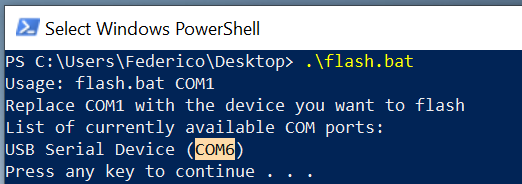
\includegraphics[width=.7\textwidth]{Chapter03/res/flashing_07.png}
	\caption{Esempio di elenco di porte COM}
	\label{fig:flashing_07}
\end{figure}

\begin{figure}[H]
	\centering
	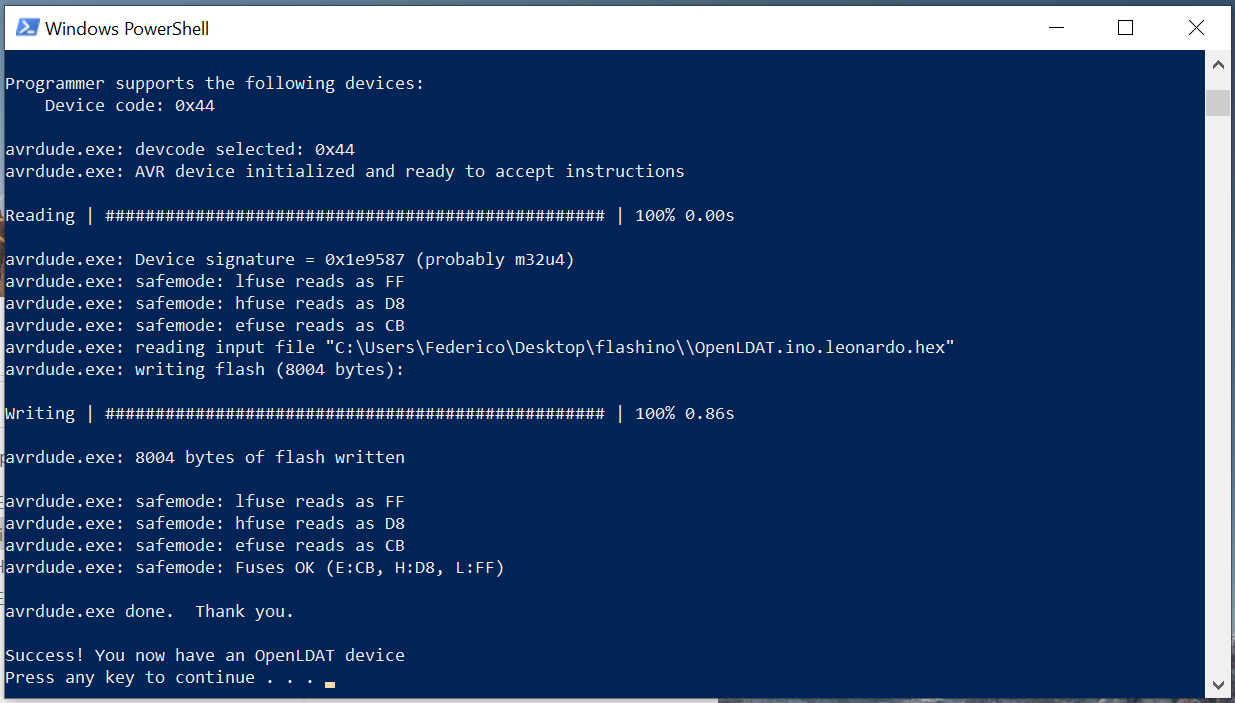
\includegraphics[width=\textwidth]{Chapter03/res/flashing_08.png}
	\caption{Output dello script automatico}
	\label{fig:flashing_08}
\end{figure}

\subsubsection{Flashing con Arduino IDE}
Il flashing con Arduino IDE è consigliato per chi vuole contribuire al progetto con modifiche al firmware.

\paragraph{Passo 1} Installare Arduino IDE. Se si sta utilizzando Windows, assicurarsi di installare anche i driver.

\paragraph{Passo 2} Aggiungere il dispositivo OpenLDAT Model 1 all'elenco delle board AVR riconosciute da Arduino IDE. Per farlo, bisogna modificare il relativo file \texttt{boards.txt}

Su Windows, il file si trova nel seguente percorso:\\
	\texttt{C:\textbackslash Program Files (x86)\textbackslash Arduino\textbackslash hardware\textbackslash arduino\textbackslash avr\textbackslash boards.txt}

Su GNU/Linux, il file si trova tipicamente in uno dei seguenti percorsi (dipende dalla distribuzione utilizzata):\\
	\texttt{/usr/share/arduino/hardware/arduino/avr/boards.txt}\\
	\texttt{/usr/share/arduino/hardware/archlinux-arduino/avr/boards.txt}\\
	\texttt{/usr/share/arduino/hardware/arduino/boards.txt}

Su MacOS, il file si trova nel seguente percorso:\\
	\texttt{\textasciitilde/Library/Arduino/hardware/arduino/avr/boards.txt}

Una volta localizzato il file, aggiungere il seguente listato alla fine del file e salvare.
\lstinputlisting{Chapter03/res/boards.txt}

\paragraph{Passo 3} Collegare il dispositivo da flashare e avviare Arduino IDE. Se è stato fatto tutto correttamente, dovrebbe essere possibile selezionare il dispositivo dall'elenco di porte seriali (figura \ref{fig:flashing_03}) e dovrebbe essere possibile selezionare come modello il dispositivo OpenLDAT Model 1 (figura \ref{fig:flashing_04}).

\paragraph{Passo 4} Aprire il gestore delle librerie di Arduino IDE e scaricare la libreria HID-Project di NicoHood (figura \ref{fig:flashing_06}). Qualora non fosse disponibile, è inclusa una copia della libreria nel file \texttt{Libraries.zip} nella cartella del firmware, che può essere estratta nella cartella libraries di Arduino.

\paragraph{Passo 5} Caricare il progetto \texttt{OpenLDAT} presente nella cartella del firmware in Arduino IDE e premere il pulsante Upload (figura \ref{fig:flashing_05}). A questo punto il dispositivo è flashato e pronto all'uso.

Attenzione: su alcune distribuzioni GNU/Linux è necessario dare al proprio utente i permessi per accedere alle porte seriali o eseguire Arduino IDE con sudo per poter flashare il dispositivo.

Attenzione: è raro ma possibile che il nome della porta seriale assegnata al dispositivo cambi durante il flashing facendolo fallire. Arduino IDE tenterà di rimediare questa cosa, ma se non riesce si può riprovare con un'altra porta USB o un altro PC.

Attenzione: il flashing con Arduino IDE introduce il problema della riproducibilità delle build. A seconda della versione del compilatore GCC e delle librerie Arduino, il firmware potrebbe essere eseguito a velocità leggermente diverse da quelle che si aspetta l'applicazione senza che questa abbia modo di saperlo. Sebbene questo non alteri significativamente le misurazioni eseguite dall'applicazione (c'è una differenza dell'1-2\%), è bene esserne a conoscenza.

\begin{figure}[H]
	\centering
	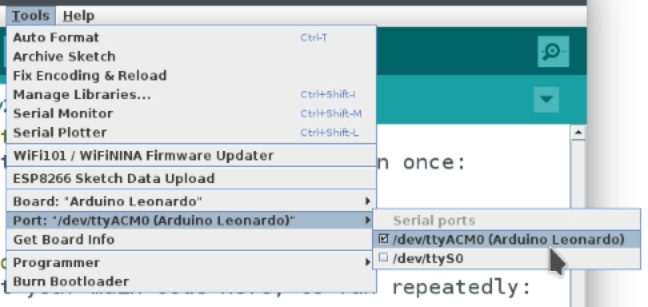
\includegraphics[width=\textwidth]{Chapter03/res/flashing_03.png}
	\caption{Selezione del dispositivo (potrebbe avere un nome diverso da Arduino Leonardo, dipende dal bootloader caricato in fabbrica)}
	\label{fig:flashing_03}
\end{figure}

\begin{figure}[H]
	\centering
	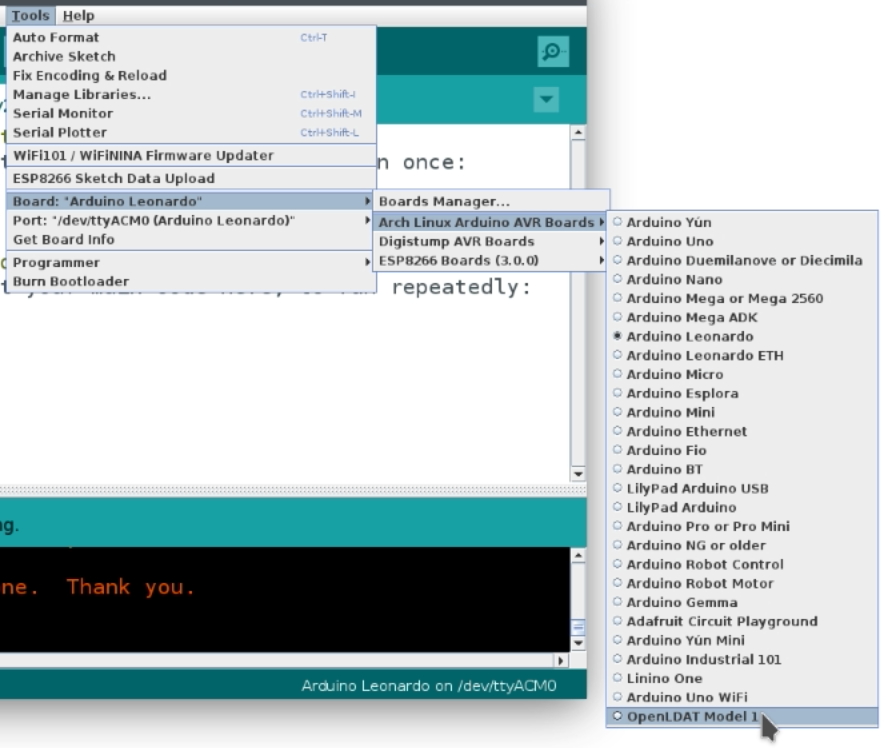
\includegraphics[width=\textwidth]{Chapter03/res/flashing_04.png}
	\caption{Selezione del modello}
	\label{fig:flashing_04}
\end{figure}

\begin{figure}[H]
	\centering
	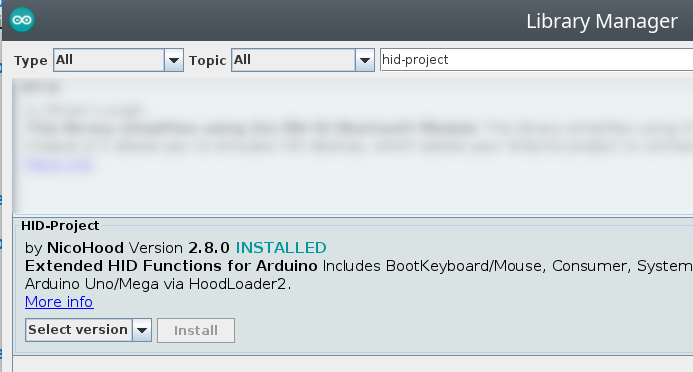
\includegraphics[width=\textwidth]{Chapter03/res/flashing_06.png}
	\caption{Download della libreria HID-Project}
	\label{fig:flashing_06}
\end{figure}

\begin{figure}[H]
	\centering
	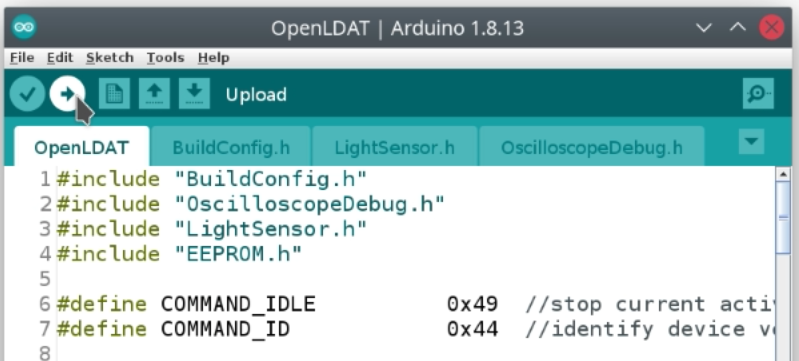
\includegraphics[width=\textwidth]{Chapter03/res/flashing_05.png}
	\caption{Pronto a flashare}
	\label{fig:flashing_05}
\end{figure}

Questo conclude il capitolo sulla parte fisica del progetto OpenLDAT. Nei capitoli successivi l'attenzione si sposterà principalmente sul software. %La parte spirituale non verrà trattata in questa tesi.
